\documentclass[11pt,]{article}
\usepackage{lmodern}
\usepackage{amssymb,amsmath}
\usepackage{ifxetex,ifluatex}
\usepackage{fixltx2e} % provides \textsubscript
\ifnum 0\ifxetex 1\fi\ifluatex 1\fi=0 % if pdftex
  \usepackage[T1]{fontenc}
  \usepackage[utf8]{inputenc}
\else % if luatex or xelatex
  \ifxetex
    \usepackage{mathspec}
  \else
    \usepackage{fontspec}
  \fi
  \defaultfontfeatures{Ligatures=TeX,Scale=MatchLowercase}
\fi
% use upquote if available, for straight quotes in verbatim environments
\IfFileExists{upquote.sty}{\usepackage{upquote}}{}
% use microtype if available
\IfFileExists{microtype.sty}{%
\usepackage{microtype}
\UseMicrotypeSet[protrusion]{basicmath} % disable protrusion for tt fonts
}{}
\usepackage[margin = 1.5in]{geometry}
\usepackage{hyperref}
\PassOptionsToPackage{usenames,dvipsnames}{color} % color is loaded by hyperref
\hypersetup{unicode=true,
            pdftitle={Linear Programming},
            pdfauthor={Abhinav Anand, IIMB},
            colorlinks=true,
            linkcolor=blue,
            citecolor=magenta,
            urlcolor=red,
            breaklinks=true}
\urlstyle{same}  % don't use monospace font for urls
\usepackage{color}
\usepackage{fancyvrb}
\newcommand{\VerbBar}{|}
\newcommand{\VERB}{\Verb[commandchars=\\\{\}]}
\DefineVerbatimEnvironment{Highlighting}{Verbatim}{commandchars=\\\{\}}
% Add ',fontsize=\small' for more characters per line
\usepackage{framed}
\definecolor{shadecolor}{RGB}{248,248,248}
\newenvironment{Shaded}{\begin{snugshade}}{\end{snugshade}}
\newcommand{\KeywordTok}[1]{\textcolor[rgb]{0.13,0.29,0.53}{\textbf{#1}}}
\newcommand{\DataTypeTok}[1]{\textcolor[rgb]{0.13,0.29,0.53}{#1}}
\newcommand{\DecValTok}[1]{\textcolor[rgb]{0.00,0.00,0.81}{#1}}
\newcommand{\BaseNTok}[1]{\textcolor[rgb]{0.00,0.00,0.81}{#1}}
\newcommand{\FloatTok}[1]{\textcolor[rgb]{0.00,0.00,0.81}{#1}}
\newcommand{\ConstantTok}[1]{\textcolor[rgb]{0.00,0.00,0.00}{#1}}
\newcommand{\CharTok}[1]{\textcolor[rgb]{0.31,0.60,0.02}{#1}}
\newcommand{\SpecialCharTok}[1]{\textcolor[rgb]{0.00,0.00,0.00}{#1}}
\newcommand{\StringTok}[1]{\textcolor[rgb]{0.31,0.60,0.02}{#1}}
\newcommand{\VerbatimStringTok}[1]{\textcolor[rgb]{0.31,0.60,0.02}{#1}}
\newcommand{\SpecialStringTok}[1]{\textcolor[rgb]{0.31,0.60,0.02}{#1}}
\newcommand{\ImportTok}[1]{#1}
\newcommand{\CommentTok}[1]{\textcolor[rgb]{0.56,0.35,0.01}{\textit{#1}}}
\newcommand{\DocumentationTok}[1]{\textcolor[rgb]{0.56,0.35,0.01}{\textbf{\textit{#1}}}}
\newcommand{\AnnotationTok}[1]{\textcolor[rgb]{0.56,0.35,0.01}{\textbf{\textit{#1}}}}
\newcommand{\CommentVarTok}[1]{\textcolor[rgb]{0.56,0.35,0.01}{\textbf{\textit{#1}}}}
\newcommand{\OtherTok}[1]{\textcolor[rgb]{0.56,0.35,0.01}{#1}}
\newcommand{\FunctionTok}[1]{\textcolor[rgb]{0.00,0.00,0.00}{#1}}
\newcommand{\VariableTok}[1]{\textcolor[rgb]{0.00,0.00,0.00}{#1}}
\newcommand{\ControlFlowTok}[1]{\textcolor[rgb]{0.13,0.29,0.53}{\textbf{#1}}}
\newcommand{\OperatorTok}[1]{\textcolor[rgb]{0.81,0.36,0.00}{\textbf{#1}}}
\newcommand{\BuiltInTok}[1]{#1}
\newcommand{\ExtensionTok}[1]{#1}
\newcommand{\PreprocessorTok}[1]{\textcolor[rgb]{0.56,0.35,0.01}{\textit{#1}}}
\newcommand{\AttributeTok}[1]{\textcolor[rgb]{0.77,0.63,0.00}{#1}}
\newcommand{\RegionMarkerTok}[1]{#1}
\newcommand{\InformationTok}[1]{\textcolor[rgb]{0.56,0.35,0.01}{\textbf{\textit{#1}}}}
\newcommand{\WarningTok}[1]{\textcolor[rgb]{0.56,0.35,0.01}{\textbf{\textit{#1}}}}
\newcommand{\AlertTok}[1]{\textcolor[rgb]{0.94,0.16,0.16}{#1}}
\newcommand{\ErrorTok}[1]{\textcolor[rgb]{0.64,0.00,0.00}{\textbf{#1}}}
\newcommand{\NormalTok}[1]{#1}
\usepackage{graphicx,grffile}
\makeatletter
\def\maxwidth{\ifdim\Gin@nat@width>\linewidth\linewidth\else\Gin@nat@width\fi}
\def\maxheight{\ifdim\Gin@nat@height>\textheight\textheight\else\Gin@nat@height\fi}
\makeatother
% Scale images if necessary, so that they will not overflow the page
% margins by default, and it is still possible to overwrite the defaults
% using explicit options in \includegraphics[width, height, ...]{}
\setkeys{Gin}{width=\maxwidth,height=\maxheight,keepaspectratio}
\IfFileExists{parskip.sty}{%
\usepackage{parskip}
}{% else
\setlength{\parindent}{0pt}
\setlength{\parskip}{6pt plus 2pt minus 1pt}
}
\setlength{\emergencystretch}{3em}  % prevent overfull lines
\providecommand{\tightlist}{%
  \setlength{\itemsep}{0pt}\setlength{\parskip}{0pt}}
\setcounter{secnumdepth}{0}
% Redefines (sub)paragraphs to behave more like sections
\ifx\paragraph\undefined\else
\let\oldparagraph\paragraph
\renewcommand{\paragraph}[1]{\oldparagraph{#1}\mbox{}}
\fi
\ifx\subparagraph\undefined\else
\let\oldsubparagraph\subparagraph
\renewcommand{\subparagraph}[1]{\oldsubparagraph{#1}\mbox{}}
\fi

%%% Use protect on footnotes to avoid problems with footnotes in titles
\let\rmarkdownfootnote\footnote%
\def\footnote{\protect\rmarkdownfootnote}

%%% Change title format to be more compact
\usepackage{titling}

% Create subtitle command for use in maketitle
\newcommand{\subtitle}[1]{
  \posttitle{
    \begin{center}\large#1\end{center}
    }
}

\setlength{\droptitle}{-2em}

  \title{Linear Programming}
    \pretitle{\vspace{\droptitle}\centering\huge}
  \posttitle{\par}
    \author{Abhinav Anand, IIMB}
    \preauthor{\centering\large\emph}
  \postauthor{\par}
      \predate{\centering\large\emph}
  \postdate{\par}
    \date{2018/07/02}

\linespread{1.25}
\usepackage{amsmath}

\begin{document}
\maketitle

\section{Background}\label{background}

Linear programming involves maximizing or minimizing a linear objective
function subject to linear inequality constraints.

\subsection{Illustration 1:}\label{illustration-1}

We consider a trivial example: suppose the objective function is
\(f(x) = 2x\) and suppose that \(x\) is constrained to be a positive
number not more than 5. More formally,

\[
\text{max } 2x: x\leq 5, x>0
\] While this is clearly an admissible linear program, it's fairly
trivial to solve. Since \(2x\) is linear and monotonic in \(x\), its
solution will occur at the end point of \(x=5\) where it attains its
maximum of 10.

\subsection{Illustration 2:}\label{illustration-2}

For a linear program whose objective function has two variables,
consider a classic portfolio analysis problem: bonds generate 5\%
returns, stocks generate 8\% returns. The total budget is \$1000. How
much of each asset should be bought?

We can translate this problem into a linear programming problem:

\[
\text{max } 0.05b+0.08s: b+s\leq 1000, b \geq 0, s \geq 0
\] where \(b, s\) respectively are the amount (in dollars) invested in
bonds and stocks.

\subsubsection{The Feasible Set}\label{the-feasible-set}

Any combination of bonds and stocks that satisfies the inequalities:
\(b ,s \geq 0\) and \(b+s\leq 1000\) is \emph{feasible}. In the problem
above, the feasible set is the following triangular region:

\begin{Shaded}
\begin{Highlighting}[]
\NormalTok{b <-}\StringTok{ }\DecValTok{0}\OperatorTok{:}\DecValTok{1000}
\NormalTok{s <-}\StringTok{ }\DecValTok{1000} \OperatorTok{-}\StringTok{ }\NormalTok{b}

\KeywordTok{ggplot}\NormalTok{(}\KeywordTok{data.frame}\NormalTok{(}\KeywordTok{cbind}\NormalTok{(b, s)), }\KeywordTok{aes}\NormalTok{(b, s)) }\OperatorTok{+}
\StringTok{  }\KeywordTok{geom_line}\NormalTok{() }\OperatorTok{+}
\StringTok{  }\KeywordTok{geom_vline}\NormalTok{(}\DataTypeTok{xintercept =} \DecValTok{0}\NormalTok{) }\OperatorTok{+}\StringTok{ }\CommentTok{#vertical line}
\StringTok{  }\KeywordTok{geom_hline}\NormalTok{(}\DataTypeTok{yintercept =} \DecValTok{0}\NormalTok{) }\OperatorTok{+}\StringTok{ }\CommentTok{#horizontal line}
\StringTok{  }\KeywordTok{theme_minimal}\NormalTok{()}
\end{Highlighting}
\end{Shaded}

\begin{center}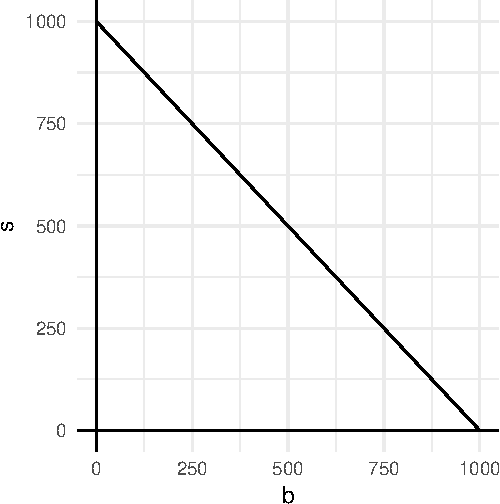
\includegraphics{Linear_Programming_files/figure-latex/plot_feasible-1} \end{center}

In the problem above and more generally, in any linear programming
problem, the feasible set is an intersection of \emph{half-spaces}.
Clearly, the more constraints we have, the smaller the feasible set is.
The feasible set in general can be of three varieties:

\begin{enumerate}
\def\labelenumi{\arabic{enumi}.}
\tightlist
\item
  It is empty. In this case there is no solution.
\item
  It is not empty but the objective function is unbounded over it.
  (\(f(x)\in\{\infty,-\infty\}\).)
\item
  It is not empty \emph{and} the objective function is bounded over it.
  (\(f(x)\in (\infty,-\infty)\).)
\end{enumerate}

Only the last case has practical value.

\subsubsection{Finding the Maximum}\label{finding-the-maximum}

In principle, to find the maximum, all we need to do is to evaluate the
objective function at all feasible points; and then see which point
yields the maximum. Clearly, this is not practical since there are a
continuum of points in this case.

The key idea is to consider a sequence of contour lines for the
objective function. Here we consider the family of lines
\(0.05b + 0.08s = \{20,35,50,\hdots\}\) etc. Then we consider which of
these intersect with our feasible set. The maximum of the objective
function will be attained at a \emph{corner point}. (Can you see why?
Hint: See illustration 1.)

\begin{Shaded}
\begin{Highlighting}[]
\NormalTok{x_b <-}\StringTok{ }\DecValTok{0}\OperatorTok{:}\DecValTok{1000}

\NormalTok{y_}\DecValTok{20}\NormalTok{ <-}\StringTok{ }\NormalTok{(}\DecValTok{20}\OperatorTok{-}\FloatTok{0.05}\OperatorTok{*}\NormalTok{x_b)}\OperatorTok{/}\FloatTok{0.08}
\NormalTok{y_}\DecValTok{35}\NormalTok{ <-}\StringTok{ }\NormalTok{(}\DecValTok{35}\OperatorTok{-}\FloatTok{0.05}\OperatorTok{*}\NormalTok{x_b)}\OperatorTok{/}\FloatTok{0.08}
\NormalTok{y_}\DecValTok{50}\NormalTok{ <-}\StringTok{ }\NormalTok{(}\DecValTok{50}\OperatorTok{-}\FloatTok{0.05}\OperatorTok{*}\NormalTok{x_b)}\OperatorTok{/}\FloatTok{0.08}
\NormalTok{y_}\DecValTok{65}\NormalTok{ <-}\StringTok{ }\NormalTok{(}\DecValTok{65}\OperatorTok{-}\FloatTok{0.05}\OperatorTok{*}\NormalTok{x_b)}\OperatorTok{/}\FloatTok{0.08}
\NormalTok{y_}\DecValTok{80}\NormalTok{ <-}\StringTok{ }\NormalTok{(}\DecValTok{80}\OperatorTok{-}\FloatTok{0.05}\OperatorTok{*}\NormalTok{x_b)}\OperatorTok{/}\FloatTok{0.08}

\NormalTok{data_plot_w <-}\StringTok{ }\KeywordTok{cbind}\NormalTok{(x_b, y_}\DecValTok{20}\NormalTok{, }
\NormalTok{                     y_}\DecValTok{35}\NormalTok{, y_}\DecValTok{50}\NormalTok{, }
\NormalTok{                     y_}\DecValTok{65}\NormalTok{, y_}\DecValTok{80}\NormalTok{) }\OperatorTok
\StringTok{  }\NormalTok{dplyr}\OperatorTok{::}\KeywordTok{as_tibble}\NormalTok{() }\CommentTok{#wide format}

\NormalTok{data_plot_l <-}\StringTok{ }\NormalTok{tidyr}\OperatorTok{::}\KeywordTok{gather}\NormalTok{(data_plot_w, }
\NormalTok{                             y_}\DecValTok{20}\OperatorTok{:}\NormalTok{y_}\DecValTok{80}\NormalTok{,}
                             \DataTypeTok{key =} \StringTok{"variables"}\NormalTok{,}
                             \DataTypeTok{value =} \StringTok{"obj_fun_values"}\NormalTok{) }\CommentTok{#long format}

\KeywordTok{ggplot}\NormalTok{(}\DataTypeTok{data =}\NormalTok{ data_plot_l, }\KeywordTok{aes}\NormalTok{(x_b, obj_fun_values)) }\OperatorTok{+}
\StringTok{  }\KeywordTok{geom_line}\NormalTok{(}\KeywordTok{aes}\NormalTok{(}\DataTypeTok{color =}\NormalTok{ variables)) }\OperatorTok{+}
\StringTok{  }\KeywordTok{geom_vline}\NormalTok{(}\DataTypeTok{xintercept =} \DecValTok{0}\NormalTok{) }\OperatorTok{+}
\StringTok{  }\KeywordTok{geom_hline}\NormalTok{(}\DataTypeTok{yintercept =} \DecValTok{0}\NormalTok{) }\OperatorTok{+}
\StringTok{  }\KeywordTok{geom_abline}\NormalTok{(}\KeywordTok{aes}\NormalTok{(}\DataTypeTok{intercept =} \DecValTok{1000}\NormalTok{, }\DataTypeTok{slope =} \OperatorTok{-}\DecValTok{1}\NormalTok{)) }\OperatorTok{+}
\StringTok{  }\KeywordTok{theme_minimal}\NormalTok{()}
\end{Highlighting}
\end{Shaded}

\begin{center}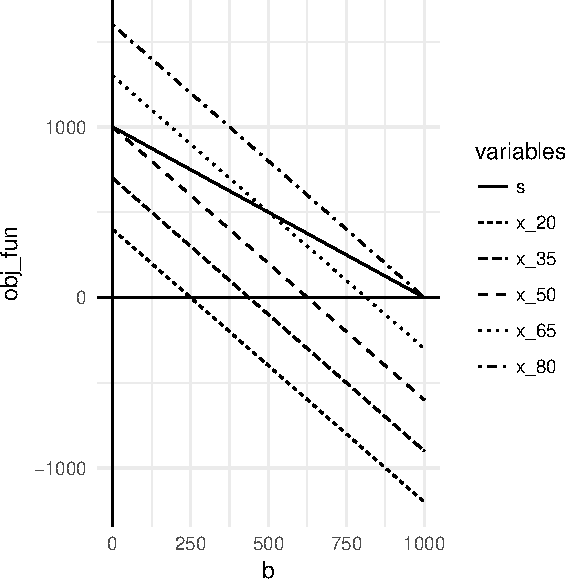
\includegraphics{Linear_Programming_files/figure-latex/plot_contour-1} \end{center}

This plot suggests that the optimal cannot occur at a strictly interior
point in the feasible set and that it must occur at some corner
point.\footnote{In general the solution could occur along some edge as
  well.} This is simple to see since the contour lines increase steadily
upwards. This yields a tempting tentative solution which computes the
objective function at all (finitely many) corners and just compares all
values to find the optimal. However, for general problems, there could
be several million corner points and this approach does not scale. Hence
we prefer to reach the maximum in a more systematic way.

\subsection{The Simplex Idea}\label{the-simplex-idea}

Devised by George Dantzig, the simplex method relies on a simple
insight: for a canonical cost minimization program, look for an optimal
solution by starting from a corner and visiting some accessible corner
with lower cost until we reach a corner for which there is no accessible
corner with cost any lower.

\subsubsection{Corners}\label{corners}

In Illustration 1, we have to maximize \(2x: x\leq 5, x>0\). (What (if
any) are the corner(s) here?) In one-dimension (\(x\in \mathbb{R}\)),
corners are merely end points. The problem above has a corner at
\(x=5\). (Is \(x=0\) also a corner?)

In two dimensions, corners are intersection points of two lines. This is
clearly the case in Illustration 2 which possesses three corners: (0,0),
(1000,0) and (0,1000).

In three dimensions corners are intersection points of three
planes---for example, ceiling corners are intersections of the three
walls (planes).

Similarly in \(n\) dimensions corners are intersections of \(n\)
hyperplanes. In general for a linear program there are \(n+m\choose n\)
possible corners. Hence brute-force evaluation of the objective function
over all corners is rendered impractical.

\section{Linear Programming: Simplex}\label{linear-programming-simplex}

Consider the canonical cost minimization linear program for two
variables, say \(x_1, x_2\):

\[
\min\{c_1x_1+c_2x_2\}: 
\] \[
a_{11}x_1+a_{12}x_2 \geq b_1
\] \[
a_{21}x_1+a_{22}x_2 \geq b_2
\] \[
x_1, x_2 \geq 0
\]

Or in vector notation:

\[
\min c^{\top}x:
\] \[
Ax\geq b, x\geq 0
\]

where \(c = (c_1, c_2), x =(x_1, x_2), b = (b_1, b_2)\) and the matrix
\(A\) is the \(2\times 2\) matrix of \(a_{ij}\).

In general,
\(c = (c_1, c_2, \hdots, c_n), x =(x_1, x_2, \hdots, x_n), b = (b_1, b_2, \hdots, b_m)\);
and \(A\) is \(m\times n\). However the general form remains the same:

\[
\min c^{\top}x:
\] \[
Ax\geq b, x\geq 0
\]

\subsection{Locating a Starting
Corner}\label{locating-a-starting-corner}

In the general formulation of the canonical cost minimization linear
program, where \(x\in \mathbb{R}^n\), at a typical corner there are
\(n\) edges that connect it to an adjacent corner. The simplex idea is
to compute the values of the objective function at the accessible
corners and choose the next one that has cost lower than that of the
current corner. Then at the next corner, repeat the process and choose
another less costly corner. Eventually there will be a special corner
all of whose adjacent corners are more expensive. This is the optimal as
reached by the simplex method.

Corners are simply the intersection points of inequalities. In general
there are \(n\) inequalities from the \(x \geq 0\) constraints and \(m\)
inequalities from \(Ax\geq b\) leading to a total of \(n+m\)
inequalities.

\subsubsection{Slack Variables}\label{slack-variables}

In Illustration 2, the inequality could be re-written after the
introduction of an auxiliary ``slack'' variable \(w\):

\[
b+s\leq 1000, b, s\geq 0 \iff b+s+w = 1000, b, s, w\geq 0
\] This transforms the inequalities \(Ax\geq 0\) to \(A\tilde{x} = 0\)
where \(\tilde{x} = (x, w)\); while retaining the other inequalities in
the form \((x, w) = \tilde{x}\geq 0\). As may be seen, the slack
variables \(w = Ax-b\) turn ``loose'' inequalities into ``tight''
inequalities (equations). The new costs become \(\tilde{c} = (c, 0)\).

The new linear program now becomes:

\[
\max  (c, 0)^{\top}(x,w): Ax - Iw = b, (x, w) \geq 0 
\] or, \[
\max \tilde{c}^{\top}\tilde{x}: [A -I]\begin{bmatrix}x\\w\end{bmatrix} = b, 
\begin{bmatrix}x\\w\end{bmatrix} \geq 0
\] or, simply without loss of generality,

\[
\max c^{\top}x: Ax = b, x \geq 0
\]

This is a general canonical form of a linear program. The equality
constraints are \(Ax=b\) and the inequality constraints are \(x\geq 0\).
There are still \(n+m\) inequalities but the slack variables have moved
them from \(Ax\geq b\) to \(x\geq 0\). The augmented vector now is
\(x = (x_1,\hdots, x_n, w_1, \hdots, w_m)\).

\subsubsection{Starting Corner}\label{starting-corner}

Translating the idea of a corner into algebra, we say that a corner of
the feasible set occurs when exactly \(n\) out of the \(n+m\) components
of \(x\) equal 0. These are exactly the \emph{basic feasible} solutions
of \(Ax = b\). Basic variables are computed by solving \(Ax = b\) and
free free components of \(x\) are set to 0.\footnote{`Basic', if \(n\)
  components equal 0; and `feasible' if \(x\geq 0\). While solving
  \(Ax=b\) (with \(A_{(m+n)\times n}\) and \(b_{m\times 1}\)) after
  Gaussian elimination there will be left exactly \(m\) pivots and \(n\)
  free variables. We stipulate the free variables to be all 0; and
  confirm if all pivots are at least 0. If so, we have a basic feasible
  solution.}

Once the starting corner is found, we move along the edge to an adjacent
corner with lower cost.

\section{Duality}\label{duality}

Every linear programming problem (called the \emph{primal} problem, with
\(x\in\mathbb{R}^n\)) can be converted into a \emph{dual} problem (with
\(y\in\mathbb{R}^m\)) the solution of which provides an upper bound for
the solution of the primal.

\textbf{Primal }: \(\max\{c^{\top} x\}: Ax\leq b, x\geq 0\)

The dual problem contains the same fundamental building blocks
\(A, b, c\) but reverses everything: in the primal, \(c\) captures the
costs while \(b\) contains the constraints. In the dual problem, \(b\)
enters the objective function and \(c\) forms the constraints. Also, if
the primal is a maximization program, its dual is a minimization
program.

\textbf{Dual}: \(\min\{b^{\top}y\}: A^{\top}y \geq c, y\geq 0\)

There are two fundamental ideas in duality:

\begin{enumerate}
\def\labelenumi{\arabic{enumi}.}
\tightlist
\item
  The dual of the dual (the so-called \emph{bidual}) is the primal. (Can
  you see how?)
\item
  Every feasible solution for a primal gives a bound on the optimal
  value for the dual.
\end{enumerate}

\subsection{Duality Theorem}\label{duality-theorem}

When primal and dual are both feasible with optimal vectors \(x^*, y^*\)
respectively, the maximum of the primal \(c^{\top}x^*\) is equal to the
minimum of the dual \(b^{\top}y^*\).

\subsubsection{Weak Duality Theorem}\label{weak-duality-theorem}

If \(x\) and \(y\) are feasible in the primal and dual respectively,
then \(c^{\top}x\leq b^{\top}y\).

In plain language, the maximal primal value is no more than the minimal
dual value for feasible points
(\(x\in \mathbb{R}^n, y\in \mathbb{R}^m\)).

\emph{Sketch of Proof}: Suppose \(x\in \mathbb{R}^n, y\in \mathbb{R}^m\)
are feasible. Then \(x:Ax\leq b\) and \(y:A^{\top}y\geq c\). Also, since
\(x, y \geq 0\), we can construct inner products and preserve the
inequalities.\footnote{Recall that for \(a,b\in \mathbb{R}^n\), the
  inner product is \(a^{\top}b=b^{\top}a=\sum a_ib_i\).}

\begin{enumerate}
\def\labelenumi{\arabic{enumi}.}
\tightlist
\item
  \(y^{\top}Ax \leq y^{\top}b\), from the primal constraints
\item
  \(x^{\top}A^{\top}y \geq x^{\top}c\), from the dual constraints. Since
  inner products are commutative, we can rewrite it as:
  \(y^{\top}(Ax) \geq c^{\top}x\).
\end{enumerate}

Hence, \(y^{\top}b\geq y^{\top}(Ax)\geq c^{\top}x\).

Weak duality implies that if the primal (max) is unbounded then the dual
(min) is infeasible. Likewise, if the dual is unbounded, then the primal
must be infeasible.\footnote{However, it is possible for both the dual
  and the primal to be infeasible.}

To each variable in the primal space corresponds a half-space (a
constraint/inequality) to satisfy in the dual space. To each constraint
to satisfy in the primal space there exists a variable in the dual
space. The coefficients that bound the inequalities in the primal space
are used to compute the objective in the dual space. Both the primal and
the dual problems make use of the same matrix.

Additionally, since each inequality can be replaced by an equality and a
slack variable, this means each primal variable corresponds to a dual
slack variable, and each dual variable corresponds to a primal slack
variable. This relation allows us to speak about \emph{complementary
slackness}.

\subsubsection{Complementary Slackness}\label{complementary-slackness}

Take \(x = (x_1,\hdots, x_n)\) as primal feasible and
\(y = (y_1,\hdots, y_m)\) as dual feasible. Denote by
\((w_1,\hdots,w_m)\) the corresponding primal slacks and by
\((z_1,\hdots,z_n)\) the corresponding dual slacks. Then \(x^*\) and
\(y^*\) are optimal for their respective problems if and only if

\begin{enumerate}
\def\labelenumi{\arabic{enumi}.}
\tightlist
\item
  \(x^*_jz_j = 0, j \in \{1,\hdots,n\}\)
\item
  \(y^*_iw_i = 0, i \in \{1,\hdots,m\}\)
\end{enumerate}

Put simply, if some component of the primal slack is positive, then the
corresponding component of the dual variable must be zero; and if some
component of the dual slack is positive then the corresponding primal
variable is zero.

It's easy to see why this is necessary: if there is a primal slack in
maximization, (i.e., there are ``leftovers''), then additional units of
that variable have no value. Likewise, if there is slack in the dual
minimum, there must be no leftovers in the primal.

\section{Computation: Linear
Programming}\label{computation-linear-programming}

Let's reconsider the old portfolio optimization program:

\[\max 0.05b+0.08s: b+s\leq 1000, b \geq 0, s \geq 0\]

This may be rewritten as:
\[\max{} [0.05, 0.08]\begin{bmatrix}b\\s\end{bmatrix}:\]
\[[1,1]\begin{bmatrix}b\\s\end{bmatrix}\leq 1000\]
\[\begin{bmatrix}b\\s\end{bmatrix}\geq 0\]

To solve such problems, we use the library \texttt{lpSolve()} containing
the function \texttt{lp()}. The general syntax for \texttt{lp()} is:

\begin{Shaded}
\begin{Highlighting}[]
\KeywordTok{lp}\NormalTok{(}\DataTypeTok{direction =} \StringTok{"max"}\NormalTok{, }\CommentTok{#default is "min"}
   \DataTypeTok{objective.in =}\NormalTok{ ..., }\CommentTok{#the objective function coefficients}
   \DataTypeTok{const.mat =}\NormalTok{ ..., }\CommentTok{#constraint matrix }
   \DataTypeTok{const.dir =}\NormalTok{ ..., }\CommentTok{#directions of constraints: >=, <= etc.}
   \DataTypeTok{const.rhs =}\NormalTok{ ...  }\CommentTok{#the constraint Right Hand Side (RHS)}
\NormalTok{   ) }
\end{Highlighting}
\end{Shaded}

This is a well tested library and can solve small to mid-sized problems,
i.e., with several hundred variables, very efficiently. The fact that
the variables have to be greater than 0 is always implicitly assumed and
does not need to be stated.

Let's try to solve the LP above using the function \texttt{lp()} from
the package \texttt{lpSolve()}.

\begin{Shaded}
\begin{Highlighting}[]
\NormalTok{optim_port <-}\StringTok{ }\NormalTok{lpSolve}\OperatorTok{::}\KeywordTok{lp}\NormalTok{(}\DataTypeTok{direction =} \StringTok{"max"}\NormalTok{,}
                          \DataTypeTok{objective.in =} \KeywordTok{c}\NormalTok{(}\FloatTok{0.05}\NormalTok{, }\FloatTok{0.08}\NormalTok{),}
                          \DataTypeTok{const.mat =} \KeywordTok{matrix}\NormalTok{(}\KeywordTok{c}\NormalTok{(}\DecValTok{1}\NormalTok{,}\DecValTok{1}\NormalTok{), }\CommentTok{#must be matrix}
                                             \DataTypeTok{nrow =} \DecValTok{1}\NormalTok{,}
                                             \DataTypeTok{byrow =}\NormalTok{ T}
\NormalTok{                                             ),}
                          \DataTypeTok{const.dir =} \KeywordTok{c}\NormalTok{(}\StringTok{"<="}\NormalTok{, }\StringTok{"<="}\NormalTok{),}
                          \DataTypeTok{const.rhs =} \DecValTok{1000}
\NormalTok{                          )}
\end{Highlighting}
\end{Shaded}

\begin{verbatim}
## Warning in rbind(const.mat, const.dir.num, const.rhs): number of columns of
## result is not a multiple of vector length (arg 2)
\end{verbatim}

\begin{Shaded}
\begin{Highlighting}[]
\NormalTok{optim_port}\OperatorTok{$}\NormalTok{solution}
\end{Highlighting}
\end{Shaded}

\begin{verbatim}
## [1]    0 1000
\end{verbatim}

\begin{Shaded}
\begin{Highlighting}[]
\NormalTok{optim_port}\OperatorTok{$}\NormalTok{objval}
\end{Highlighting}
\end{Shaded}

\begin{verbatim}
## [1] 80
\end{verbatim}

It's easy to have guessed the solution of the above program even without
computing it formally. (How? Is there a simple way to see this?)

Here is a more involved program:

\[\max{} 25x_1+20x_2: \] \[20x_1+12x_2\leq 1800\]
\[1/15x_1+1/15x_2\leq 8\] \[x_1,x_2\geq 0\]

\begin{Shaded}
\begin{Highlighting}[]
\NormalTok{optim_lp <-}\StringTok{ }\NormalTok{lpSolve}\OperatorTok{::}\KeywordTok{lp}\NormalTok{(}\DataTypeTok{direction =} \StringTok{"max"}\NormalTok{,}
                        \DataTypeTok{objective.in =} \KeywordTok{c}\NormalTok{(}\DecValTok{25}\NormalTok{, }\DecValTok{20}\NormalTok{),}
                        \DataTypeTok{const.mat =} \KeywordTok{matrix}\NormalTok{(}\KeywordTok{c}\NormalTok{(}\DecValTok{20}\NormalTok{, }\DecValTok{12}\NormalTok{, }\DecValTok{1}\OperatorTok{/}\DecValTok{15}\NormalTok{, }\DecValTok{1}\OperatorTok{/}\DecValTok{15}\NormalTok{),}
                                           \DataTypeTok{nrow =} \DecValTok{2}\NormalTok{,}
                                           \DataTypeTok{byrow =}\NormalTok{ T),}
                        \DataTypeTok{const.dir =} \KeywordTok{c}\NormalTok{(}\StringTok{"<="}\NormalTok{, }\StringTok{"<="}\NormalTok{),}
                        \DataTypeTok{const.rhs =} \KeywordTok{c}\NormalTok{(}\DecValTok{1800}\NormalTok{, }\DecValTok{8}\NormalTok{)}
\NormalTok{                        )}

\NormalTok{optim_lp}\OperatorTok{$}\NormalTok{solution}
\end{Highlighting}
\end{Shaded}

\begin{verbatim}
## [1] 45 75
\end{verbatim}

\begin{Shaded}
\begin{Highlighting}[]
\NormalTok{optim_lp}\OperatorTok{$}\NormalTok{objval}
\end{Highlighting}
\end{Shaded}

\begin{verbatim}
## [1] 2625
\end{verbatim}

\section{Application: Quantile
Regressions}\label{application-quantile-regressions}

Quantile regression aims to estimate the conditional median (or other
quantiles) of the dependent variable as opposed to its conditional mean,
which is the objective of an ordinary least squares exercise. Quantile
estimates, somewhat unsurprisingly, are more robust measures of
conditional dependence. Median regressions for large data sets were
unpopular until recently since they are quite tedious compared to the
least squares method.

\subsection{Mean and Medians as Optimization
Programs}\label{mean-and-medians-as-optimization-programs}

\subsubsection{Argmin of Sum of Squared
Deviations}\label{argmin-of-sum-of-squared-deviations}

Given observations \(b_1,\hdots,b_m\), find \(b\) such that the sum of
observations' squared deviations from \(b\) is minimum:

\[\min_b{} (b-b_1)^2+\hdots+(b-b_m)^2\]
\[\min_b{} \sum_{i=1}^m (b-b_i)^2\] Then
\[f(x) = \sum_{i=1}^m (x-b_i)^2\]
\[f^{\prime}(x) = \sum_{i=1}^m 2(x-b_i)\]
\[f^{\prime\prime}(x) = 2m > 0\]

Hence there is a minimum \(x^*\) such that
\[f^{\prime}(x) = \sum_{i=1}^m 2(x-b_i) = 0 \Rightarrow x^* = \frac{\sum_{i=1}^m b_i}{m}\]

Hence the mean \(x^* = \frac{\sum_{i=1}^m b_i}{m}\) minimizes the sum of
the squared distance between itself and the observations.

\subsubsection{Argmin of Sum of Absolute
Deviations}\label{argmin-of-sum-of-absolute-deviations}

Given observations \(b_1,\hdots,b_m\), find \(b\) such that the sum of
observations' absolute deviations from \(b\) is minimum:

\[\min_b{} |b-b_1|+\hdots+|b-b_m|\] \[\min_b{} \sum_{i=1}^m |b-b_i|\]
Then \[g(x) = \sum_{i=1}^m |x-b_i|\]
\[g^{\prime}(x) = \sum_{i=1}^m sgn(x-b_i)\cdot 1\]
\[g^{\prime}(x) = |\{i: b_i < x\}| - |\{i: b_i \geq x\}| \]

Hence there is a minimum \(x_*\) such that
\[g^{\prime}(x) =  0 \Rightarrow x_* = b_{\frac{1+m}{2}}\]

Hence the median \(x_* = b_{\frac{1+m}{2}}\) minimizes the sum of the
absolute distance between itself and the observations.

\subsection{Regressions: Least Squares and
Median}\label{regressions-least-squares-and-median}

In general, a least squares regression is:
\[y = X\beta+u; \text{and } \mathbb{E}(u|X) = 0\] and the problem is to
find \(\beta^*\) such that the sum of the squares of the residuals are
minimum: \[\min_{\beta}{} \|u\|_2=\min_{\beta}{}\|y-X\beta\|_2\]

where \(\|u\|_2 := \sqrt{\sum_{i=1}^m u_i^2}\) is the \emph{Euclidean}
norm (also called the \(L^2\) norm).

Analogously, a \emph{median} regression is:
\[y = X\beta_{0.50}+u; \text{and } \mathbb{Q}_{0.50}(u|X) = 0\] where
\(Q_{\tau}(Y|X)\) is the \(\tau_{\text{th}}\) conditional quantile of Y
given X and the problem is to find \(\beta_{0.50}^*\) such that the sum
of the absolute values of the residuals are minimum:
\[\min_{\beta_{0.50}}{} \|u\|_1=\min_{\beta_{0.50}}{}\|y-X\beta_{0.50}\|_1\]

where \(\|u\|_1 := \sum_{i=1}^m |u_i|\) is the \(L^1\) norm.

Hence the median regression problem is:
\[\min_{\beta_{0.50}}{} \sum_{i=1}^m |u_i|=\sum_{i=1}^m |y_i-X_i^{\top}\beta_{0.50}|\]

\subsubsection{Quantile Regression: The General
Case}\label{quantile-regression-the-general-case}

In the same way as the median, a general quantile \(\tau\in(0,1)\) for a
sequence of observations \(y_1,\hdots,y_m\) can be computed as the
minimum of the following program:
\[\min_{y_{\tau}} \{\sum_{i:y_i>y_{\tau}}|y_i-y_{\tau}|\cdot \tau +
\sum_{i:y_i\leq y_{\tau}}|y_i-y_{\tau}|\cdot (1-\tau)
\}\]

Hence the general quantile regression is:
\[\min_{\beta_{\tau}}{} \{\sum_{i:y_i>\beta_{\tau}}\tau\cdot|y_i-X_i^{\top}\beta_{\tau}|
+ \sum_{i:y_i\leq\beta_{\tau}}(1-\tau)\cdot|y_i-X_i^{\top}\beta_{\tau}|
\}\]

We can recast the above as follows:
\[u_i := \max(y_i-X_i^{\top}\beta_{\tau}, 0)\]
\[v_i := \min(y_i-X_i^{\top}\beta_{\tau}, 0)\]
\[b_{+}:= \max(\beta_{\tau}, 0)\] \[b_{-}:= \min(\beta_{\tau}, 0)\]

giving the generic following linear program:

\[\min{}\sum_{i=1}^m (\tau\cdot u_i + (1-\tau)\cdot v_i):\]
\[u_i, v_i\geq 0, i\in\mathbb{N}\] \[b_{+}, b_{-}\geq 0\]
\[y_i = X_i^{\top}(b_{+}-b_{-})+u_i-v_i\]

In matrix notation we get: \[\max{} -[0,0,\tau,1-\tau]
\begin{bmatrix}
b_{+}\\
b_{-}\\
u\\
v
\end{bmatrix}:
\] \[[X,-X,I,-I]
\begin{bmatrix}
b_{+}\\
b_{-}\\
u\\
v
\end{bmatrix}
= y\] \[b_{+},b_{-},u,v\geq 0\]

Hence in particular, for the median regression, with \(\tau=0.50\), we
have the program: \[\min \sum_{i=1}^m|y_i-y|\]
\[\min \sum_{i=1}^m (a_i+b_i):\] \[y_i-y=a_i-b_i\] \[a_i, b_i\geq 0\]

\subsection{Computation: Median
Regressions}\label{computation-median-regressions}

Find the median of a sequence of observations (residuals) which (we know
now) is the solution for the median regression problem above. We assume
the observations (residuals) are normally distributed.

\begin{Shaded}
\begin{Highlighting}[]
\NormalTok{num <-}\StringTok{ }\DecValTok{201} \CommentTok{#number of points}
\NormalTok{u <-}\StringTok{ }\KeywordTok{rnorm}\NormalTok{(num, }\DecValTok{0}\NormalTok{, }\DecValTok{1}\NormalTok{) }\CommentTok{#normal 0, 1 residuals}

\CommentTok{# One constraint per row: a[i], b[i] >= 0}
\NormalTok{A1 <-}\StringTok{ }\KeywordTok{cbind}\NormalTok{(}\KeywordTok{diag}\NormalTok{(}\DecValTok{2}\OperatorTok{*}\NormalTok{num),}\DecValTok{0}\NormalTok{)}

\CommentTok{# a[i] - b[i] = y[i] - y}
\NormalTok{A2 <-}\StringTok{ }\KeywordTok{cbind}\NormalTok{(}\KeywordTok{diag}\NormalTok{(num), }\OperatorTok{-}\KeywordTok{diag}\NormalTok{(num), }\DecValTok{1}\NormalTok{)}

\NormalTok{quant_med <-}\StringTok{ }\NormalTok{lpSolve}\OperatorTok{::}\KeywordTok{lp}\NormalTok{(}\StringTok{"min"}\NormalTok{,}
                         \KeywordTok{c}\NormalTok{(}\KeywordTok{rep}\NormalTok{(}\DecValTok{1}\NormalTok{,}\DecValTok{2}\OperatorTok{*}\NormalTok{num),}\DecValTok{0}\NormalTok{),}
                         \KeywordTok{rbind}\NormalTok{(A1, A2),}
                         \KeywordTok{c}\NormalTok{(}\KeywordTok{rep}\NormalTok{(}\StringTok{">="}\NormalTok{, }\DecValTok{2}\OperatorTok{*}\NormalTok{num), }\KeywordTok{rep}\NormalTok{(}\StringTok{"="}\NormalTok{, num)),}
                         \KeywordTok{c}\NormalTok{(}\KeywordTok{rep}\NormalTok{(}\DecValTok{0}\NormalTok{,}\DecValTok{2}\OperatorTok{*}\NormalTok{num), u)}
\NormalTok{                         )}

\NormalTok{quant_med}\OperatorTok{$}\NormalTok{solution }\OperatorTok\StringTok{ }\KeywordTok{tail}\NormalTok{()}
\end{Highlighting}
\end{Shaded}

\begin{verbatim}
## [1] 0.4333183 0.8685031 0.2651384 0.0000000 0.0000000 0.0000000
\end{verbatim}

\begin{Shaded}
\begin{Highlighting}[]
\KeywordTok{median}\NormalTok{(u)}
\end{Highlighting}
\end{Shaded}

\begin{verbatim}
## [1] -0.1095907
\end{verbatim}


\end{document}
